
\chapter{METHODOLOGY}
{\baselineskip=2\baselineskip

In this chapter, the researchers outline the methodology employed to conduct the study, providing a comprehensive overview of the research design, technical design workflow, and analytical procedures.

\section{Research Design and Procedure}

\begin{figure}[H]
	\centering
	\caption{The Waterfall Model}
	\label{fig:waterfall}
	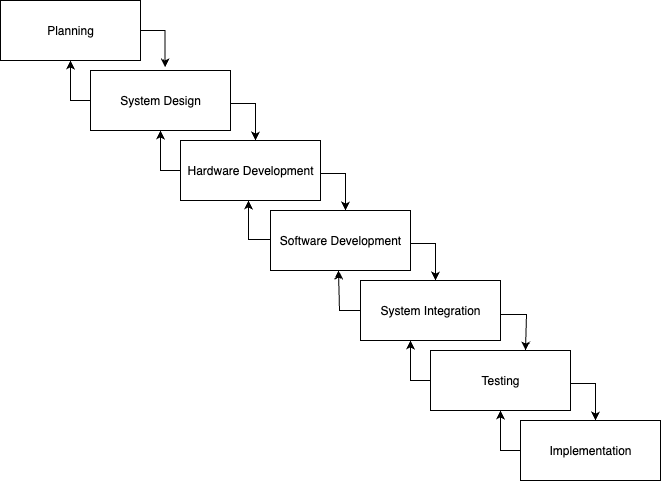
\includegraphics[width=1\textwidth]{figures/waterfall.png}
\end{figure}

In Figure 3.1, the system creation process is illustrated, utilizing a modified waterfall model. This systematic approach consists of several key stages, commencing with requirements gathering and followed by requirements analysis, hardware development, software development, system design, integration, and testing \& evaluation. This procedural framework acts as a guiding path for researchers to achieve the study's intended objectives.


\subsection{Research Setting}

\begin{figure}[H]
	\centering
	\caption{Map of Camiguin and Misamis Oriental}
	\label{fig:map}
	\includegraphics[width=0.6\textwidth]{figures/map.png}
\end{figure}

The research will be conducted in selected areas of Camiguin and Misamis Oriental, regions in the Philippines that are known for frequent and unscheduled power interruptions. These areas are served by CAMELCO (Camiguin Electric Cooperative) and MORESCO II (Misamis Oriental Electric Cooperative II), both of which experience regular power outages, particularly during peak hours. This issue disrupts daily activities, especially in community centers, educational institutions, and local businesses that rely on electricity for mobile devices, lighting, and small appliances.


\subsection{Data Collection}

The research team will gather data from both primary and secondary sources. For the primary data, first-hand interactions will be conducted with community residents, power supply providers, and solar energy experts. Community residents, as the primary users of the solar-powered rental station, will provide information on the demand for portable power sources, willingness to adopt a solar-powered system, and feedback on system usability and effectiveness in addressing power interruptions. Power supply providers, such as local electric cooperatives like CAMELCO and MORESCO 2, will provide data on the frequency of power interruptions, challenges in accessing reliable energy, and the overall energy demand in the community. Insights from solar energy experts will focus on technical aspects of solar power systems, including optimal photovoltaic panel configurations, energy storage solutions, and power inverter specifications.

Secondary sources will include academic papers, case studies, industry reports, and other literature related to solar energy, portable power stations, and renewable energy systems. These sources will provide a theoretical foundation and context for the study, ensuring that both practical relevance and technical feasibility are considered in developing the solar-powered rental station system.

\subsection{Data Gathering Procedure}

To obtain relevant qualitative data for the study, a series of in-depth interviews will be conducted with selected community residents using purposive sampling. The interviews will focus on understanding residents’ experiences with frequent power interruptions, the challenges they encounter during interruptions, and their perceptions of a solar-powered rental station with detachable power source as an alternative energy source. These discussions will also explore their reliance on backup power systems and their willingness to adopt renewable energy solutions. Participants will be purposively selected, particularly those who frequently experience power interruptions, depend on electricity for livelihood activities, and have expressed interest in solar technology. Combined with qualitative tools, this approach will ensure a comprehensive understanding of the community’s energy needs, user expectations, and potential areas for improving the design and implementation of the solar-powered rental station system.

\subsection{Data Finding Analysis}

The analysis of the collected data will lead to several important findings. The first will reveal that community residents frequently experience power interruptions that disrupt both household and livelihood activities. These interruptions will highlight common challenges related to the reliability, cost, and accessibility of backup power solutions. Residents will express concerns about their dependence on the unstable power grid and the lack of affordable alternatives during interruptions. The analysis will also uncover the community’s openness to adopting a solar-powered rental solution, recognizing its potential to provide a more sustainable and reliable energy source. Feedback from interviews and discussions will emphasize the need for practical improvements to the proposed system, such as flexible payment options (coin- or app-based), increased power capacity, and user-friendly accessibility. These insights will be vital in assessing the system’s feasibility and refining its design to ensure it effectively addresses the residents’ energy needs.

\subsection{User Definition}

After the planning phase, the system’s users were identified. For this study, the Community Resident is defined as follows:

\textit{Community Resident - A person residing in a local community who is actively involved or has access to the portable power sources during power interruptions or emergencies.}

\subsection{System Requirements}

	\begin{longtable}{|p{4cm} | p{9cm}|}
		\caption{System Requirements} \label{tab:long} \\
		
		\hline \multicolumn{1}{|c|}{\textbf{Category}} & \multicolumn{1}{c|}{\textbf{System Requirement}} \\ \hline 
		\endfirsthead
		
		\multicolumn{2}{c}%
		{{\bfseries \tablename\ \thetable{} -- continued from previous page}} \\
		\hline \multicolumn{1}{|c|}{\textbf{Category}} & \multicolumn{1}{c|}{\textbf{System Requirement}}  \\ \hline 
		\endhead
		
		\hline \multicolumn{2}{|r|}{{Continued on next page}} \\ \hline
		\endfoot
		
		\endlastfoot
	
	Input Requirements & - The system shall collect user information during account registration through designated input fields in the mobile application. \\
	& - The system shall accept user login credentials such as username and password for authentication. \\
	& - The system shall accept rental requests, including power source selection, rental duration, and payment method (coin-based or app-based).\\
	& - The system shall receive telemetry data from each power source, including battery percentage, GPS location, and rental status through the GSM module. \\
	& - The system shall receive telemetry data from each power source, including battery percentage, GPS location, and rental status through the GSM module.  \\
	\hline
		
	Process Requirements & - The system shall process rental transactions by verifying payment completion before authorizing power source access. \\
	& - The system shall generate and transmit an access token or unlock code to the power source upon successful rental approval. \\
	& - The system shall continuously monitor and record the battery level, location, and usage duration of active rentals. \\
	& - The system shall automatically send an SMS notification via GSM one hour before the allotted 12-hour usage period ends, and if the user exceeds the 12-hour limit, it shall continue sending overdue alerts every 10 minutes until the item is returned. \\
	& - The system shall process the return of rented power sources by validating device ID, updating the database, and releasing the final transaction summary. \\
	& - The system shall calculate credit earned for users based on unused power and reflect the updated balance in the users mobile application account. \\
	\hline
		
	Output Requirements & - The system shall display rental confirmation details such as power source ID, rental duration, and current charge level. \\
	& - The system shall provide updates on the detachable power source, provide user logs, and notify the admin whenever a new account is created. \\
	& - The system shall generate the location of the rented power source using the GSM module. \\
	& - The system shall generate notifications on the mobile app, including GPS location, and rental time remaining. \\
	& - The system shall calculate the unused power of the returned detachable power source and convert it into a credit stored in the user’s mobile app. \\
	\hline
	
	Control Requirements & - The system shall implement user authentication and authorization mechanisms to restrict access to registered users only. \\
	& - The system shall validate all rental and payment data to ensure that only completed and legitimate transactions are processed. \\
	\hline
	
	Performance Requirements & - The system shall maintain fast response time during login, payment processing, and rental activation to ensure a smooth user experience. \\
	& - The system shall provide monitoring and synchronization of power source data through reliable GSM and IoT communication.\\
	& - The system shall ensure continuous operation and high availability to prevent service interruptions during rentals. \\
	\hline
	
\end{longtable} 


\subsection{Calculation Requirements}

\subsubsection{Load Analysis}

\begin{longtable}{p{3cm} p{1.9cm} p{1.4cm} p{2.3 cm} p{4cm}}
	\caption{Load Consumption} \label{tab:LoadConsumption} \\
	\toprule
	\textbf{Load} & \textbf{Quantity} & \textbf{Power} & \textbf{Hours/Day} & \textbf{Daily Consumption} \\
	\midrule
	\endfirsthead
	
	\toprule
	\textbf{Load} & \textbf{Quantity} & \textbf{Power} & \textbf{Hours/Day} & \textbf{Daily Consumption} \\
	\midrule
	\endhead
	
	\bottomrule
	\endfoot
	
	Electric Fan & 1 & 75 W & 5 & 370 WH \\
	Mobile Phone Charger & 1 & 20 W & 5 & 100 WH \\
	Auxiliary Load & 1 & 5 W & 5 & 25 WH \\
	\midrule
	\textbf{Total} & & & & \textbf{500 WH} \\
\end{longtable}

The schedule of load includes three main loads, namely the electric fan, the mobile phone charger, and a 5W auxiliary load. Each load is multiplied by its hours of operation, and their products are summed to obtain the total watt-hour daily consumption. 

All calculations are done in accordance to PEC (Philippine Electrical Code 2017).

\subsubsection{Battery Sizing}

\begin{itemize}
	\item\textbf{ Detachable Power Source:} 
	\begin{equation}
		\text{Battery Capacity} =
		\left( \frac{\text{Total Daily Consumption}}{\text{System Voltage}} \right)
		+ \text{ESP32 Consumption}
		\label{eq:batterysizing}
	\end{equation}
	
	
	This equation determines the required battery capacity for the detachable power source. The total daily load consumption in watt-hours is divided by the 12V system voltage to convert the value into ampere-hours. The consumption of the ESP32 microcontroller (0.858 Ah), which continuously operates for system monitoring, is then added. This computation ensures that the detachable power source can sustain both the primary load and the microcontroller’s operational requirements. Please refer to \hyperref[appendix:A]{Appendix A} for the detailed computation.
	
	\item\textbf{ Station:} 
	\begin{equation}
		\text{Battery Capacity} =
		\left( 
		\text{BCDPS}
		+ 35\%
		\right)
		+ \text{ESP32 Consumption}
		\label{eq:Station}
	\end{equation}
	
	
	This equation is used in sizing the battery of the main station. It begins with the computed battery capacity of the detachable power source and adds 35\% to account for system losses, such as wiring resistance, power conversion inefficiencies, and charging losses. The ESP32’s consumption (0.858 Ah) is also included to ensure that the main station battery can support all monitoring and control operations. Please refer to \hyperref[appendix:A]{Appendix A} for the detailed computation.
	
	\item\textbf{ Panel Sizing:} 
	\begin{equation}
		\text{PV Power} =
		\frac{\text{Total Daily Consumption}}{\text{Sun Peak Hours}}
		\label{eq:panel}
	\end{equation}
	
	
	This equation calculates the required power rating of the solar panel. The total daily energy consumption (500 Wh) is divided by the available sun peak hours (3.5 hours, based on PEC 2017) to determine the power output needed to fully recharge the battery each day. The computed value of approximately 142.86W is rounded up to a 200W solar panel for practical and technical considerations. Please refer to \hyperref[appendix:A]{Appendix A} for the detailed computation.
	
	\item \textbf{Inverter Sizing:} 
	\begin{longtable}{p{4cm} p{1.5cm} p{2.5cm} p{4cm}}
		\caption{Inverter Sizing} \label{tab:InverterSizing} \\
		\toprule
		\textbf{Load} & \textbf{Power} & \textbf{Power Surge} & \textbf{With Power Surge} \\
		\midrule
		\endfirsthead
		
		\toprule
		\textbf{Load} & \textbf{Power} & \textbf{Power Surge} & \textbf{With Power Surge} \\
		\midrule
		\endhead
		
		\bottomrule
		\endfoot
		
		Electric Fan & 75 W & 3 & 225 W \\
		Mobile Phone Charger & 20 W & 1 & 20 W \\
		Auxiliary Load & 5 W & 1 & 5 W \\
		\midrule
		\textbf{Total} & & & \textbf{250 W} \\
	\end{longtable}
	\begin{equation}
		\text{Inverter Size} =
		\text{Total Power Consumption} + 20\% \text{Allowance}
		\label{eq:inverter}
	\end{equation}
	
	
	This formula is used to determine the appropriate inverter size. After calculating the total power requirements of all connected loads, including surge components such as the electric fan, a 20\% allowance is added to ensure that the inverter can safely handle fluctuations and temporary increases in power demand. With a total of 250W, the system requires a 300W pure sine wave inverter. Please refer to \hyperref[appendix:A]{Appendix A} for the detailed computation.
	
	\item \textbf{Solar Charge Controller Sizing:} 
	\begin{equation}
		I_{cc} =
		\frac{\text{Total PV Power}}{\text{System Voltage}}
		\label{eq:solar}
	\end{equation}
	
	
	This equation determines the required rating for the solar charge controller. Dividing the total solar panel wattage (200W) by the system voltage (12V) yields the expected charging current supplied to the controller. The computed value of 16.67A is rounded upward to select a 20A MPPT charge controller, ensuring safe and efficient power regulation. Please refer to \hyperref[appendix:A]{Appendix A} for the detailed computation.
	
	\item \textbf{Breaker Sizing:} 
	\begin{enumerate}[label=\alph*.]
		\item Panel - SCC
		\begin{equation}
			\text{Circuit Breaker} = 11.85A \times\text{Over Radiance Factor} \times \text{Safety Factor}
		\end{equation}
		
		
		This equation is used to determine the appropriate circuit breaker rating between the solar panel array and the Solar Charge Controller (SCC). The value 11.85A represents the short-circuit current (Isc) of the solar panel system. Multiplying by the Over Radiance Factor and the Safety Factor provides an adjusted current value that accounts for sudden increases in sunlight intensity and unexpected current surges.
		After substituting the given parameters in the complete computation, the calculated value results in a 20A circuit breaker rating, which is the recommended protection size between the solar panel and the SCC. This ensures safe operation by preventing overheating, protecting the solar wiring, and avoiding damage to system components. Please refer to \hyperref[appendix:A]{Appendix A} for the detailed computation.
		
		\item SCC - Battery
		\begin{equation}
			\text{Circuit Breaker} = \frac{\text{Total Array Wattage}}{\text{Battery Bank Nominal Voltage}} \times \text{Safety Factor}
		\end{equation}
		
		
		This equation sizes the circuit breaker between the Solar Charge Controller (SCC) and the battery bank. The total wattage of the solar panel array is divided by the system’s nominal battery voltage to determine the expected charging current that will flow from the SCC into the battery during operation. A Safety Factor is then applied to account for possible current variations during charging, ensuring that the system remains protected from overload.
		After substituting the system values into the calculation, the resulting breaker rating requirement is 20A, which provides proper protection during charging while maintaining safe operating conditions for the battery bank. This recommended 20A circuit breaker prevents overheating and electrical damage by limiting excessive current flow into the battery storage system. Please refer to \hyperref[appendix:A]{Appendix A} for the detailed computation.
		
		\item Battery - Power Inverter
		\begin{equation}
			\text{Circuit Breaker} = \frac{\text{Power Inverter}}{\text{Battery Bank Nominal Voltage}}
		\end{equation}
		
		
		This equation determines the appropriate circuit breaker rating between the battery bank and the power inverter. The power rating of the inverter (in watts) is divided by the nominal battery voltage (in volts) to calculate the maximum current drawn during inverter operation when supplying AC loads. This calculated current serves as the basis for selecting a circuit breaker capable of protecting both the inverter and battery system during high-demand usage.
		After substituting the specified system values into the equation, the resulting breaker requirement is 80A, which is the recommended rating to ensure sufficient protection from overcurrent conditions that may occur when connected appliances operate at maximum load capacity. This breaker rating prevents damage to the inverter and battery by interrupting excessive current flow and maintaining safe operating conditions. Please refer to \hyperref[appendix:A]{Appendix A} for the detailed computation.
		
		\item Inverter - Load (AC Breaker)
		\begin{equation}
			\text{Circuit Breaker} = \frac{ \text{Safety Load}}{\text{Inverter Voltage Output}} \times \text{BBNV}
		\end{equation}
		
		
		This equation sizes the AC circuit breaker located between the inverter and the connected load. The Safety Load represents the maximum expected power consumption of the AC appliances connected to the inverter. Dividing this value by the inverter’s AC output voltage converts the load into current, representing the expected amperage during operation. The result is then multiplied by the battery bank nominal voltage to account for conversion losses and variations in real operating conditions.
		Based on the system values used in the computation, the required AC breaker rating is 4A, which provides sufficient protection by interrupting excessive current that could damage connected appliances or the inverter output circuitry. This calculated breaker size ensures safe and reliable system performance under normal and peak load operations. Please refer to \hyperref[appendix:A]{Appendix A} for the detailed computation.
		
	\end{enumerate}
	
	\item \textbf{Wire Sizing:} 
	\begin{equation}
		\text{Voltage Drop Index} = \frac{\text{Amperes} \times \text{Wire Length (Feet)}}{\text{Voltage} \times \text{Percent Voltage Drop}}
	\end{equation}
	
	
	This equation is used for determining the appropriate wire size needed to safely and efficiently handle electrical current within the system. The Voltage Drop Index (VDI) is calculated based on four factors: the current in amperes, the wire length, the system voltage, and the allowable percentage of voltage drop. Higher current flow or longer cable distance increases the VDI value, which indicates the need for a thicker wire in order to minimize electrical resistance and heat generation. Selecting the correct wire size ensures that voltage loss is controlled, system performance remains efficient, and the overall electrical design operates safely without risk of overheating or component failure.
	
	\begin{enumerate}[label=\alph*.]
		\item Panel - SCC \\
		Panel to Solar Charge Controller = 10AWG 
		
		
		The first VDI calculation was performed for the wire connection between the solar panel and the Solar Charge Controller (SCC). Given the operational current and wire distance in this segment, the computed VDI value resulted in 3.52. Based on standard VDI wire reference charts, a value of 3.52 corresponds to the use of 10 AWG wire, which provides sufficient conductivity and prevents excessive voltage reduction over the cable length. This ensures that power harvested from the solar panel is efficiently delivered to the SCC with minimal losses. Please refer to \hyperref[appendix:A]{Appendix A} for the detailed computation.
		
		\item SCC - Battery\\
		Solar Charge Controller to Battery = 10AWG
		
		
		The second VDI calculation was conducted for the wire connection between the Solar Charge Controller (SCC) and the battery bank. Using the specified current, distance, system voltage, and allowable voltage drop percentage, the computed VDI value for this segment is 3.125. Similar to the previous result, this VDI value also aligns with the requirement for 10 AWG wire, ensuring safe current handling capacity and controlled voltage drop. The consistent selection of 10 AWG wire across both connection points maintains electrical balance and reliability throughout the charging circuit. Please refer to \hyperref[appendix:A]{Appendix A} for the detailed computation.
		
	\end{enumerate}
\end{itemize}

\section{Technical Design Workflow}
\subsection{System Architecture}

\begin{figure}[H]
	\centering
	\caption{System Architecture}
	\label{fig:architecture}
	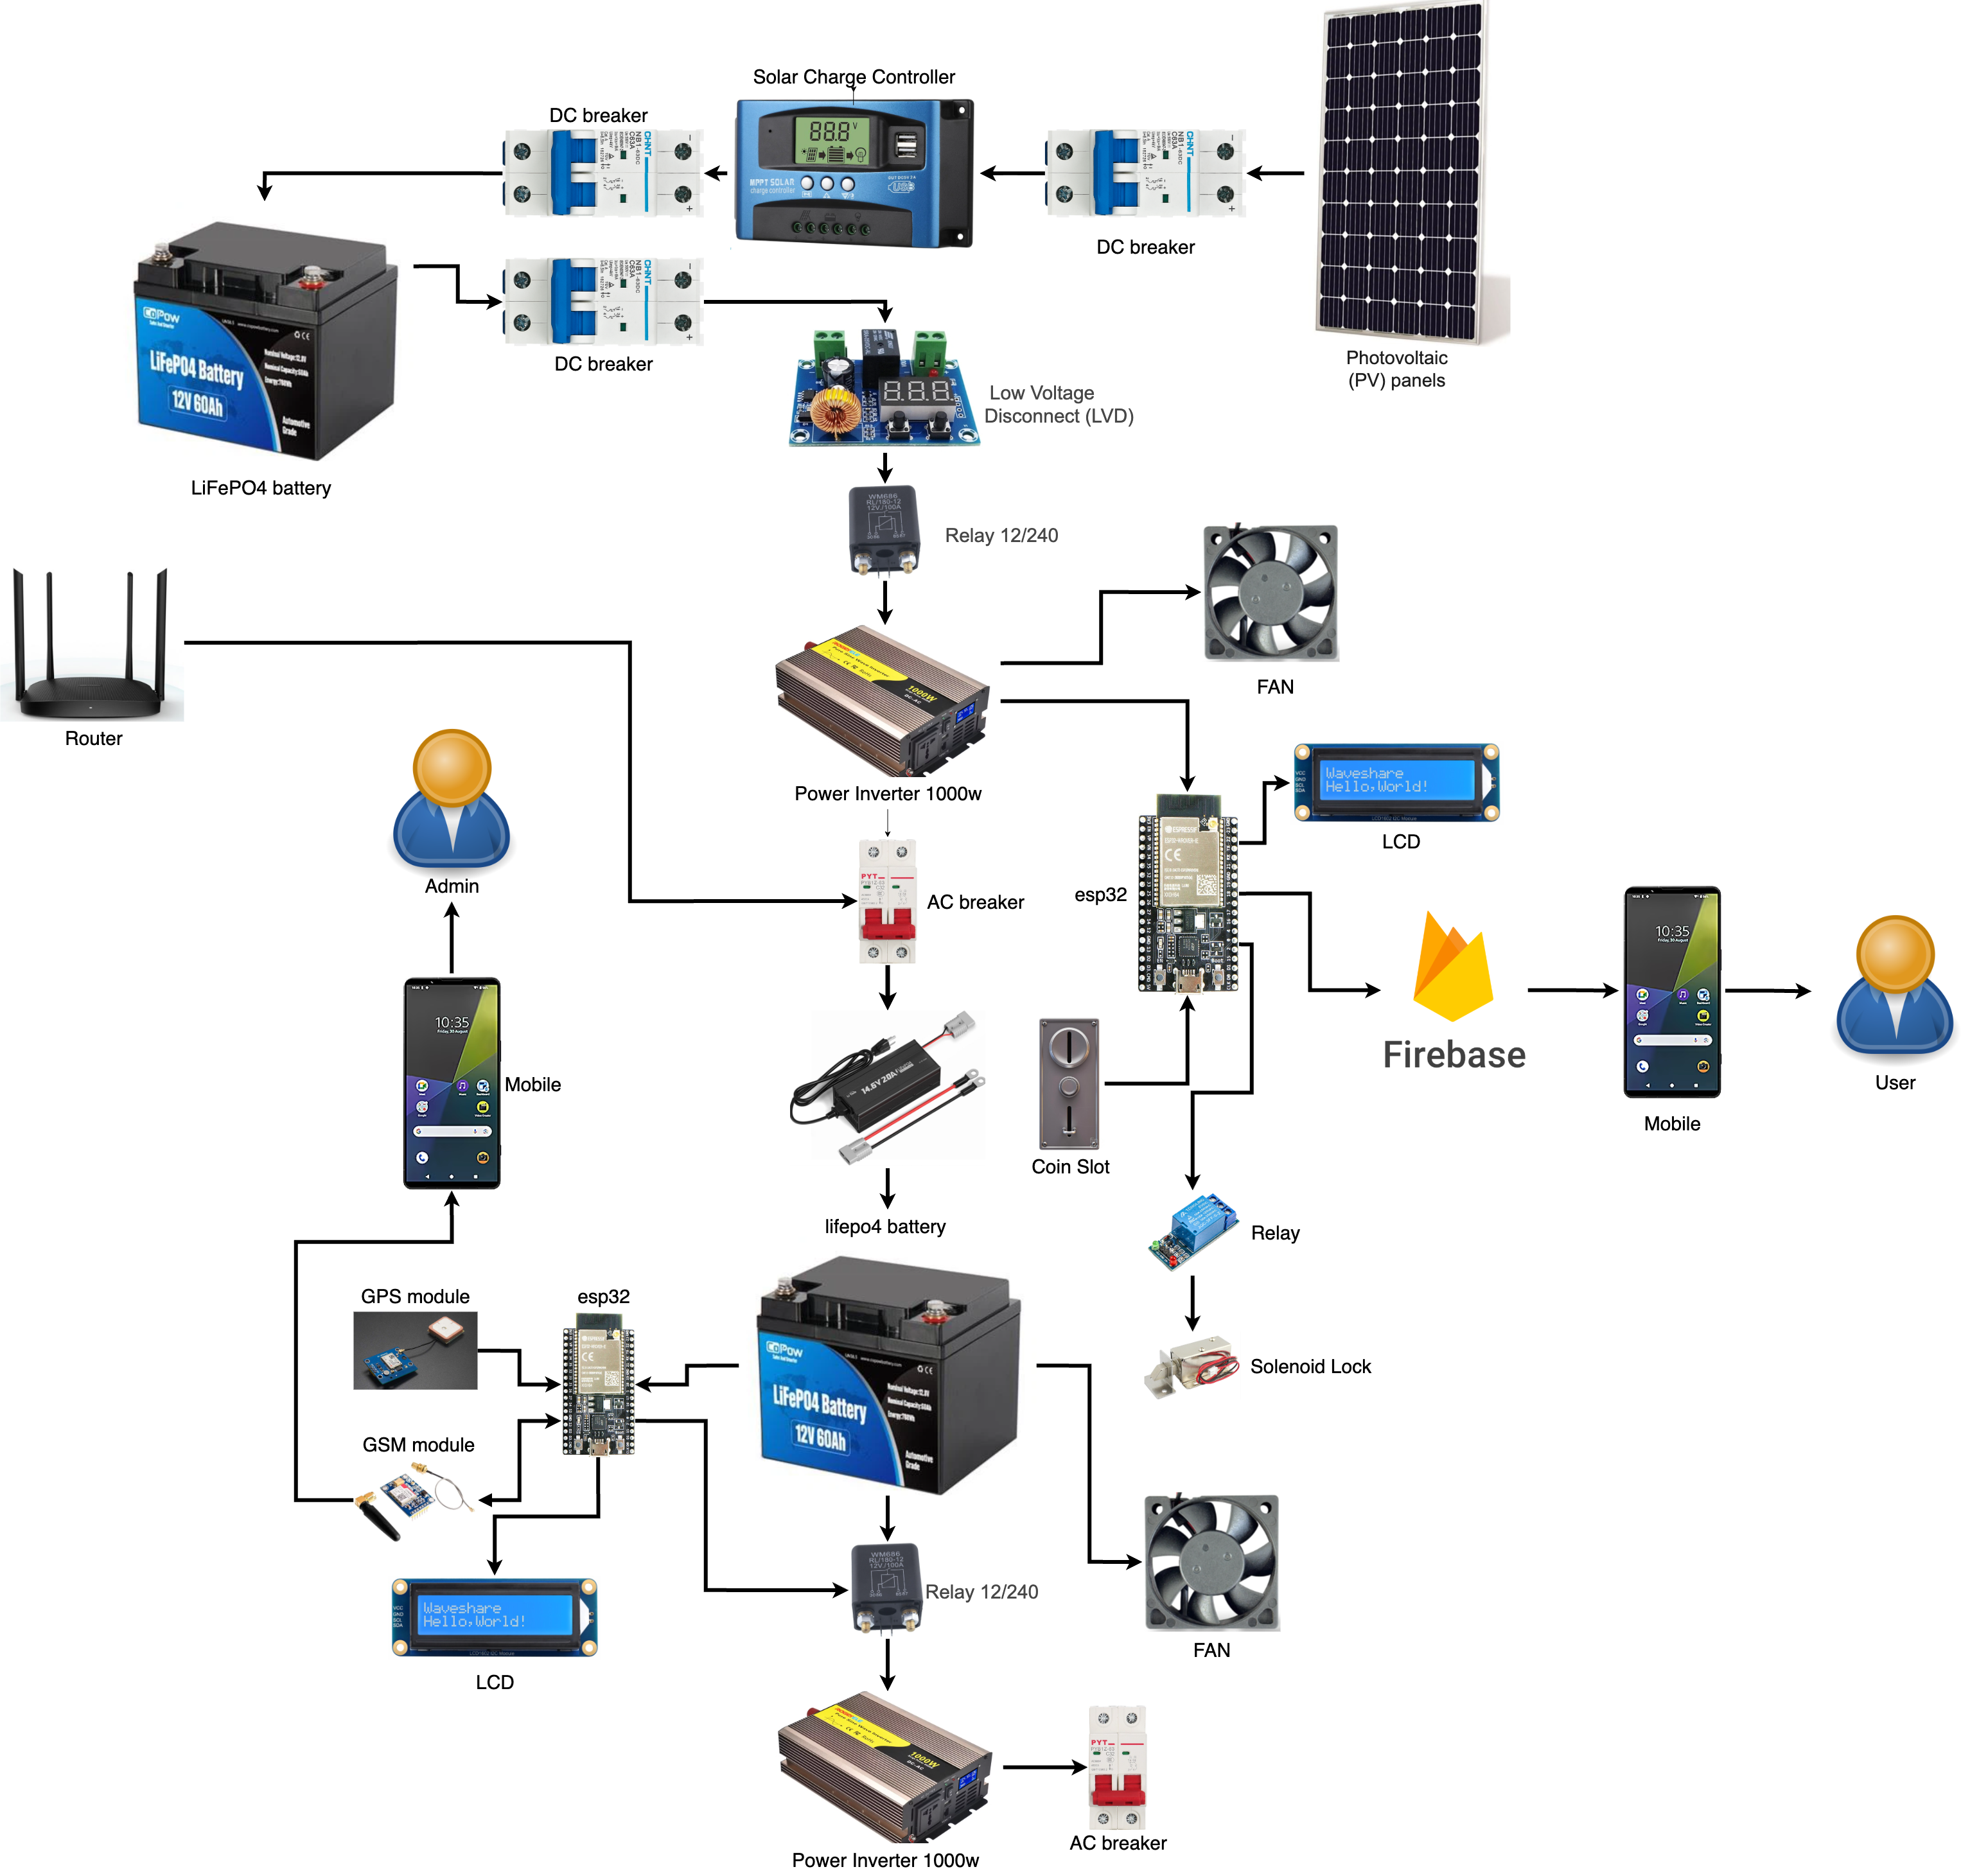
\includegraphics[width=0.85\textwidth]{figures/architecture.jpg}
\end{figure}

The Figure 3.3 illustrates the overall architecture of the solar powered rental station with a detachable power source. The system is designed to harvest solar energy, convert it to usable power, and provide access to users through various interfaces and technologies.

\begin{itemize}
	
	\item \textit{Solar Energy Collection and Storage} - PV panels capture solar energy, which is stored in a \ce{LiFePO4}  battery through a solar charge controller and DC breakers for protection.
	
	\item \textit{Energy Conversion} - The stored DC power is converted to AC using a power inverter to supply household appliances.
	
	\item \textit{User Interface and Control }- The ESP32 microcontroller connects with a mobile app via a router and Firebase, allowing users to monitor battery levels and manage rental requests.
	
	\item \textit{Power Access and Management} - A coin slot and relay control access to the power source, while an LCD displays real-time system status.
	
	\item \textit{GPS Tracking and Securit}y -  A GPS and GSM module track the power source’s location, ensuring security and preventing theft.
	
	\item \textit{Admin Control} - Admins can monitor and manage the system through a mobile interface, overseeing usage and system health.
	
\end{itemize}

This system is designed to provide a sustainable, secure, and user-friendly power source solution for communities, utilizing solar energy and modern IoT technologies for enhanced management and accessibility.

\subsection{Flowchart}
\begin{figure}[H]
	\centering
	\caption{System Flowchart}
	\label{fig:flowchart}
	\includegraphics[width=0.6\textwidth]{figures/flowchart.png}
\end{figure}

Figure 3.4 illustrates the overall process of the proposed Solar-Powered Rental Station with Detachable Power Sources. The process begins with the initialization of the ESP32, which activates system components and prepares communication protocols. The system first checks slot availability to determine if a detachable power source is ready for use. Data from this process is transmitted through the internet and stored in a central database for monitoring purposes.

When a user intends to rent a power source, the system verifies if payment is successful. If confirmed, the solenoid lock opens, allowing the detachable power source to be accessed by the user. Once rented, the ESP32 continuously monitors the power source, including its GPS location and battery percentage, and sends the information to the administrator via SMS. This ensures proper tracking and security of the rented device.

The system also monitors whether the detachable power source is returned. If it remains unreturned after 12 hours, the ESP32 automatically sends reminder SMS notifications to both the user and the administrator. Upon return, the solenoid lock closes, securing the power source back in place. All key actions, including errors and system activities, are logged in the database for reference and analysis.


\subsection{Solar Energy Harvesting}

\begin{figure}[H]
	\centering
	\caption{Conversion of Sunlight into Electrical Energy using PV Panels and a Charge Controller}
	\label{fig:solar harvesting}
	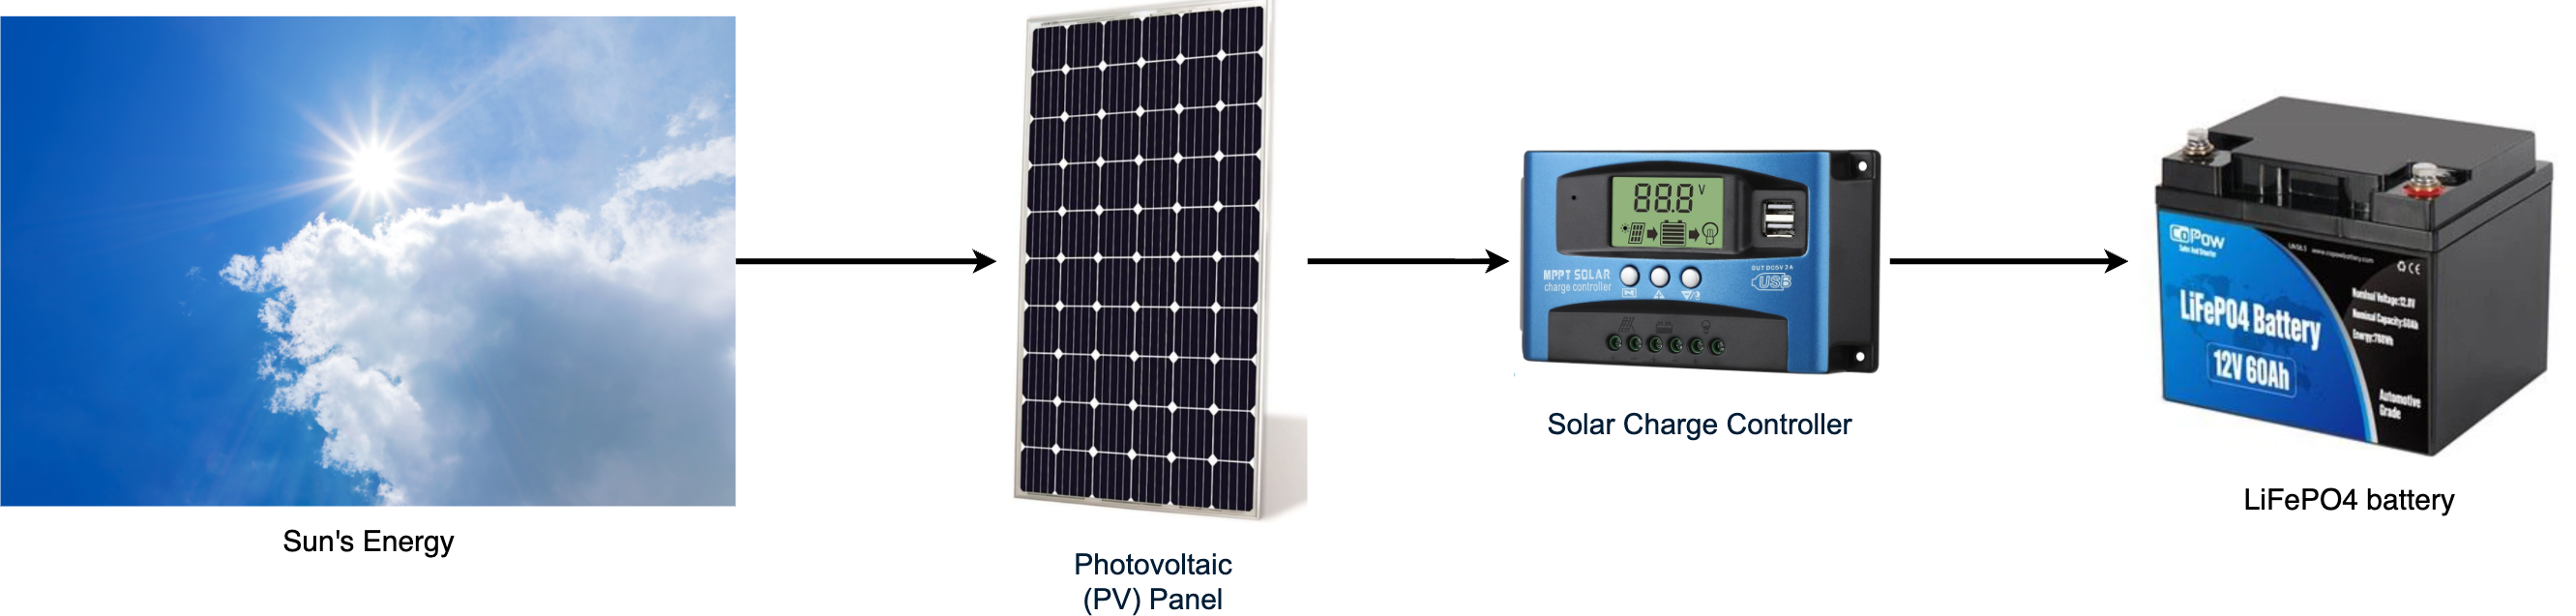
\includegraphics[width=1\textwidth]{figures/harvesting.png}
\end{figure}

The Figure 3.5 illustrates the process of harvesting solar energy using photovoltaic (PV) panels. Solar energy is captured by the PV panels, which then convert sunlight into electrical energy. The energy is stored in a \ce{LiFePO4} battery through a solar charge controller, ensuring proper charging and voltage regulation. This energy is stored for later use, contributing to the overall sustainability and efficiency of the system, enabling it to power devices even during periods of limited sunlight.

\subsection{Energy Conversion DC to AC}

\begin{figure}[H]
	\centering
	\caption{Battery DC power converted to AC output via Inverter.}
	\label{fig:energy conversion}
	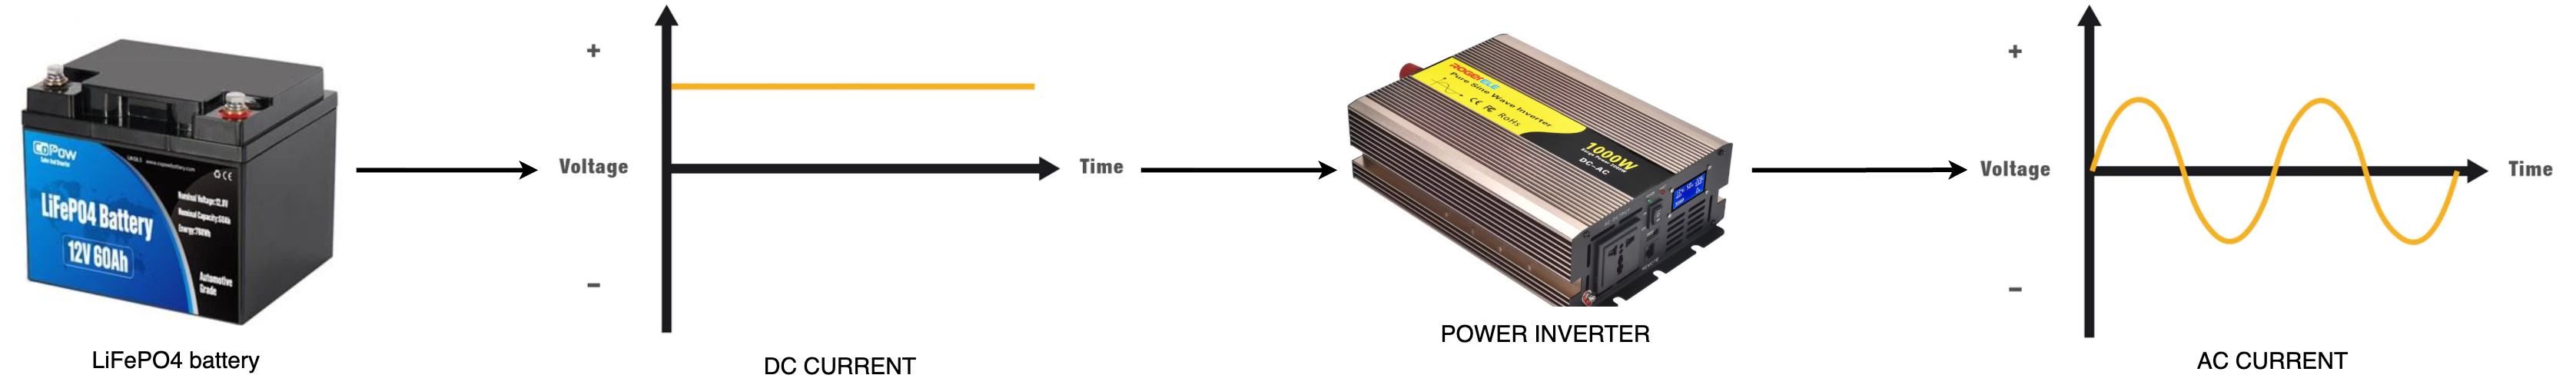
\includegraphics[width=1\textwidth]{figures/conversion.png}
\end{figure}

Figure 3.6 shows the process of converting direct current (DC) into alternating current (AC). The stored energy in the \ce{LiFePO4} battery is passed through a power inverter, and the inverter transforms the DC from the battery into AC power, which can be used to power household appliances such as fans and other AC-powered devices. This conversion is essential for making the system compatible with common electrical appliances that require AC power for operation.

\subsection{Power Monitoring}

\begin{figure}[H]
	\centering
	\caption{ESP32 measures battery voltage and displays data on LCD}
	\label{fig:power monitoring}
	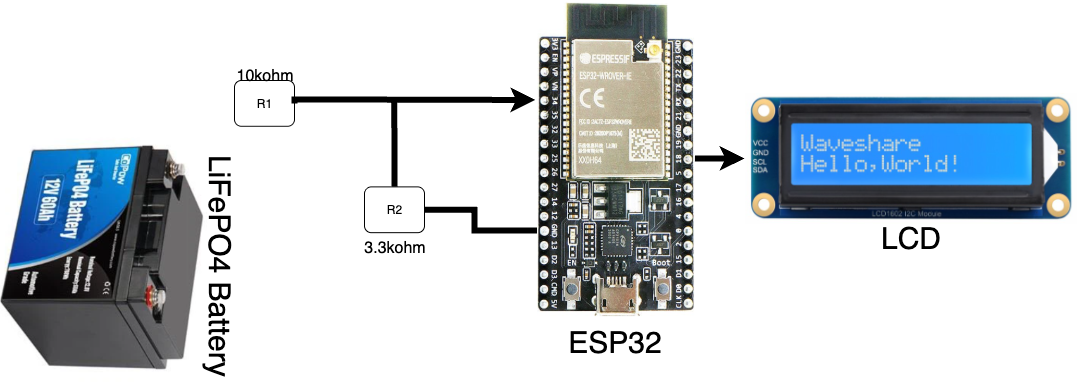
\includegraphics[width=1\textwidth]{figures/monitoring.png}
\end{figure}

The Figure 3.7 illustrates the power monitoring system used to keep track of the energy stored and consumed by the system. The \ce{LiFePO4} battery is connected to an ESP32 microcontroller, which continuously monitors the battery’s voltage and health, and the data collected is displayed on an LCD screen which allows users to view the battery's current status. This monitoring is vital for ensuring the system's efficiency and preventing over-discharge, ensuring long-term sustainability.


\subsection{GPS Tracking}

\begin{figure}[H]
	\centering
	\caption{ESP32 receives location data from GPS satellites using GSM Module}
	\label{fig:gps tracking}
	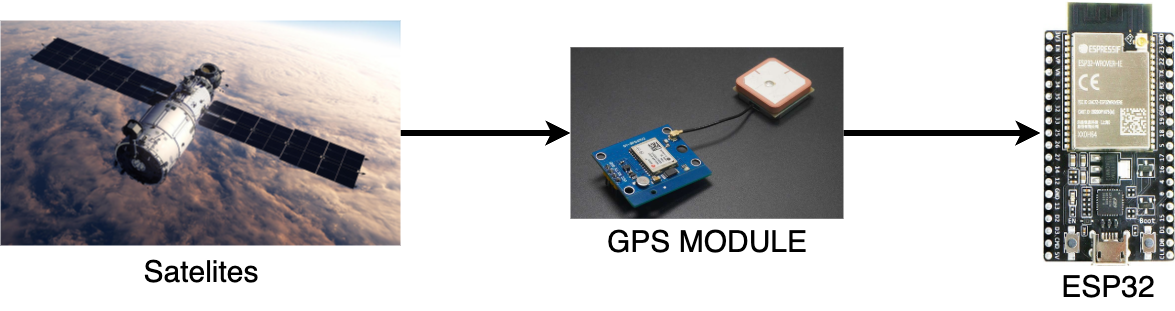
\includegraphics[width=1\textwidth]{figures/tracking.png}
\end{figure}

Figure 3.8 shows the GPS tracking system used to monitor the location of the detachable power source. A GPS module, connected to the ESP32 microcontroller, receives signals from satellites to determine the geographical location of the system. This location data is essential for tracking and managing the rental and use of the power sources, ensuring they are accessible to users and protected from theft or misuse. The GPS data is then sent to the system for further processing and user access.


\subsection{Context Level Diagram}

\begin{figure}[H]
	\centering
	\caption{Context Level Diagram}
	\label{fig:context level diagram}
	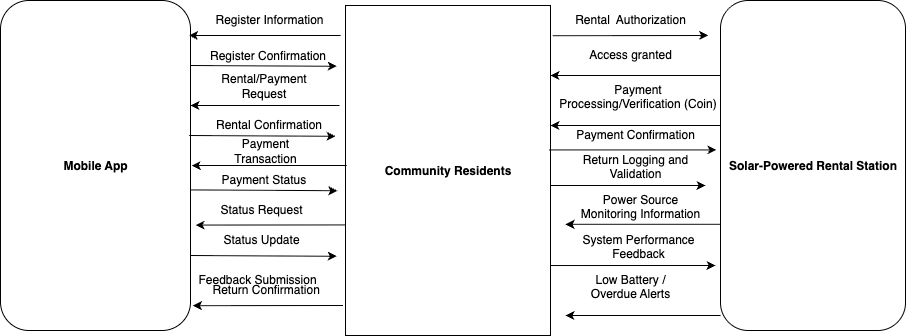
\includegraphics[width=\textwidth]{figures/context.png}
\end{figure}

This Figure 3.9 illustrates the complete interaction flow of the solar-powered rental system, showing how the Mobile App, Community Residents, Solar-Powered Rental Station, and the Detachable Power Source communicate with one another. The process begins with community residents using the mobile application to register their information, submit rental requests, process payments, and receive status updates. Once a rental request is made, the app sends the relevant information to the system, which then confirms the registration, validates the rental request, and updates the user about payment status and rental confirmation.

The interaction between the community residents and the solar-powered rental station focuses on physical access and transaction validation. The rental station authorizes the rental, verifies payment, and grants access permission for users to retrieve the detachable power source. Upon returning the device, the station logs and validates the return, ensuring that the power source is securely and correctly returned. The station then issues a return confirmation to the user, completing the rental cycle.

The detachable power source also communicates with the system to strengthen security and monitoring. It provides identification data, sends monitoring information such as location and usage status, and confirms both retrieval and return actions. These interactions ensure that the system can track each device, prevent unauthorized usage, and maintain accountability for each rental unit. Overall, the diagram presents a structured overview of how all components work together to support registration, rental, payment, monitoring, and return of the solar-powered power source in a seamless and secure manner.

\subsection{Data Flow Diagram}
\begin{figure}[H]
	\centering
	\caption{Data Flow Representation of the Solar-Powered Rental Station System}
	\label{fig:data flow}
	\includegraphics[width=1\textwidth]{figures/dflow.png}
\end{figure}
	
The Figure 3.10 shows the complete process flow of the solar-powered rental station system, illustrating how community residents interact with the mobile application and system database. It begins with the login process, where residents input their login details, which are verified by the system. Once authenticated, the system provides feedback confirming successful login. After logging in, the user proceeds to make a rental request by selecting a power source and specifying the rental duration. The system responds with rental confirmation and product details. The user then moves to the payment process, where payment details are submitted through the app. The system validates the payment, sends a confirmation, and generates an access token that authorizes the user to unlock and use the detachable power source.

Once access is granted, the rental authorization and monitoring phase begins. The system continuously provides updates on the power source’s status, such as battery level and remaining usage time, ensuring that the user can track energy consumption. When the rental period ends, the user then sends a return request, and the system verifies and confirms the return while updating the rental status. After returning the power source, the user proceeds to the feedback process, submitting performance feedback through the app. The system stores the feedback and confirms successful submission. After that, the system records the final rental summary and sends any overdue alerts if the power source is not returned on time. Overall, the diagram presents a clear and structured view of how the user’s actions and system responses are linked throughout the entire rental transaction cycle, which is from login to feedback completion.

\subsection{Use Case Diagram}
 \begin{figure}[H]
 	\centering
 	\caption{Use Case Diagram}
 	\label{fig:use case}
 	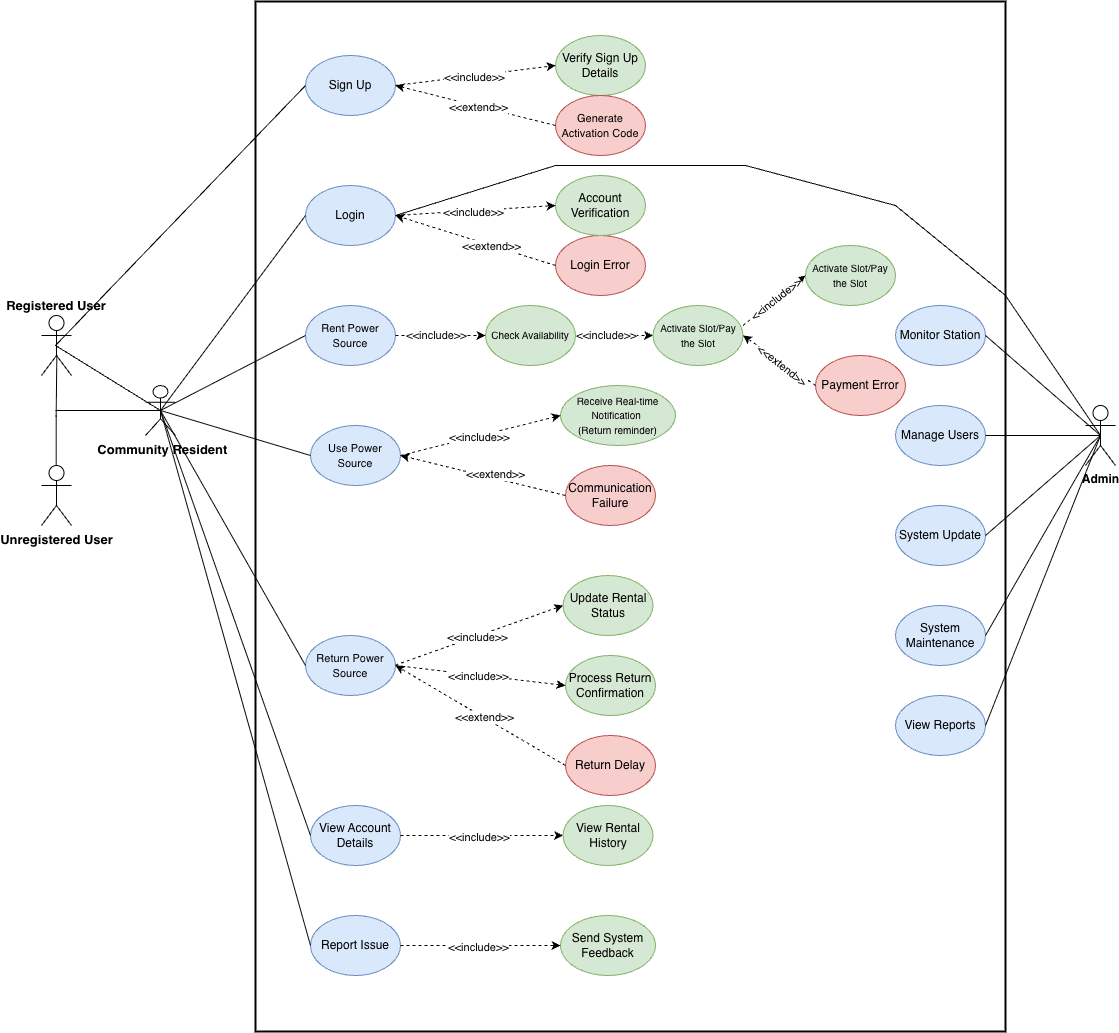
\includegraphics[width=1\textwidth]{figures/usecase.png}
 \end{figure}
 
Figure 3.11 illustrates how different users and administrators interact with the system. It highlights the actions users can take and the roles of administrators. The Unregistered User is someone who has not yet signed up for the system. They can create an account by providing their details, which are then verified by the system. If the details are correct, an activation code is generated for the user to complete the registration. After signing up, the user can log in to the system, but if there’s an issue with the login, an error is displayed.
 
 Once the Unregistered User becomes a Registered User after logging in successfully, they can perform more actions within the system. The user can rent a power source by checking its availability, paying for it, and activating the slot where the power source is stored. If there’s a problem with communication during the rental process, the system handles this as an extended action. After using the power source, the user can return it, and the system confirms the return. If there’s any delay in returning the power source, the system will manage this as well. Registered users also have the ability to view their account details and rental history, and they can report any issues or provide feedback through the system. The Admin plays a key role in overseeing the system. They can manage users, including adding or removing them from the system. The admin is also responsible for performing system updates and maintenance, ensuring the smooth operation of the system. Additionally, the admin can view various reports that provide insights into system performance and user activities.
 
 The relationships in the diagram are shown through Include and Extend. Include means that one action is always linked to another. For example, signing up always includes verifying the user's details, and renting a power source includes checking availability and processing payment. Extend means that certain actions may trigger additional steps under specific conditions. For instance, if a payment fails, it will trigger the "Payment Error" action, or if the power source return is delayed, it will trigger the "Return Delay" action. In summary, this use case diagram provides an overview of how users and administrators interact with the system, covering key actions like renting and returning power sources, managing user accounts, and maintaining the system.
 
 \subsection{Activity Diagram}
  \begin{figure}[H]
 	\centering
 	\caption{Activity Diagram of the Community Resident}
 	\label{fig:activity}
 	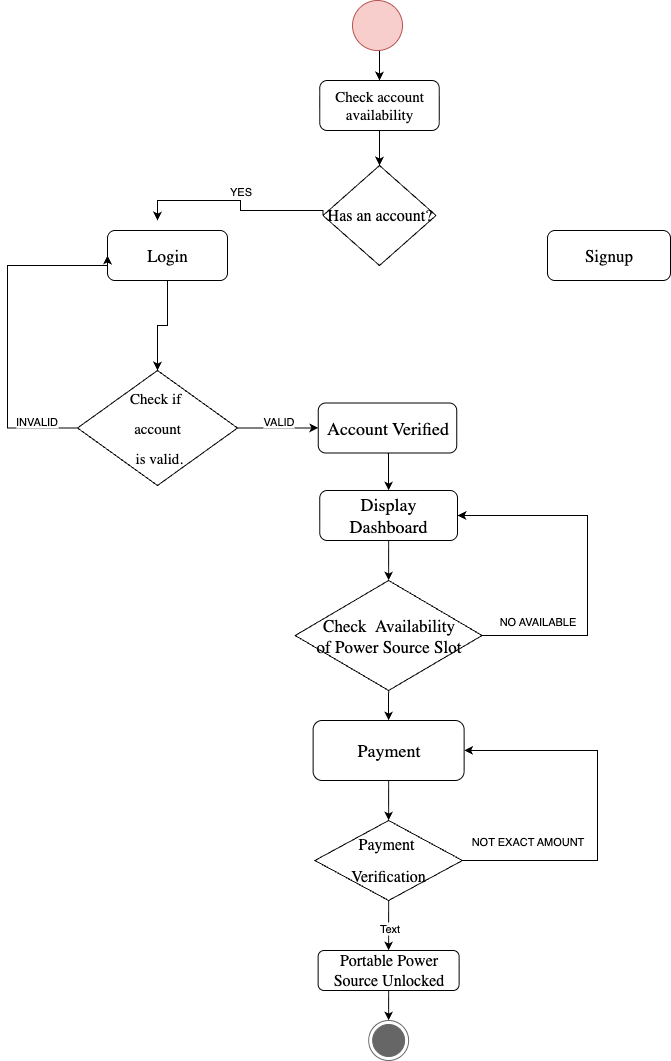
\includegraphics[width=0.55\textwidth]{figures/activity.png}
 \end{figure}
 
Figure 3.12 shows the step-by-step activity flow of the system from user login to unlocking the portable power source. The process begins with checking account availability. If the user already has an account, they proceed to the login step; otherwise, they must sign up first. After logging in, the system checks if the account is valid. If the account is invalid, the process returns to the login step. If valid, the system verifies the account and displays the dashboard. Next, the system checks if a power source slot is available. If no slot is available, the user remains on the dashboard until one becomes free. If a slot is available, the process continues to the payment step. The system then verifies the payment amount. If the amount entered is not exact, the process returns to the payment step. If the payment is correct, the portable power source is successfully unlocked, completing the process.

Overall, the diagram clearly shows how the user interacts with the system , which starts from account access, validation, and payment, up to unlocking the rented portable power source.
   
  \subsection{3D Design}
  
  The 3D representation shows the overall design of the detachable power source and the solar-powered rental station. It provides a clear visual of the system’s shape and structure. The model illustrates how the different parts of the system are arranged in space, allowing a better understanding of the physical layout of the proposed system.
  
    \begin{figure}[H]
  	\centering
  	\caption{Front View of the Power Source – Three Dimensional Representation}
  	\label{fig:3d}
  	\includegraphics[width=0.8\textwidth]{figures/front.png}
  \end{figure}
 
    \begin{figure}[H]
 	\centering
 	\caption{Aerial View of the Power Source – Three Dimensional Representation}
 	\label{fig:3d2}
 	\includegraphics[width=0.8\textwidth]{figures/aerial.png}
 \end{figure}
 
    \begin{figure}[H]
 	\centering
 	\caption{Three Dimensional Representation of the Rental Station of the Detachable Power Source}
 	\label{fig:3d3}
 	\includegraphics[width=1\textwidth]{figures/rental.png}
 \end{figure}
 
Figure 3.15 shows the 3D design of the system. It is a stationary power station powered by solar energy and contains three detachable power sources. The system has a single coin slot that controls access, and each detachable power source is secured with a solenoid lock.
  
  \subsection{Mobile App}
  
     \begin{figure}[H]
  	\centering
  	\caption{Welcome Page}
  	\label{fig:welcome}
  	\includegraphics[width=1\textwidth]{figures/welcome.png}
  \end{figure}
  
  The welcome interface presents the system logo and entry actions. The left panel shows a splash screen with a “Get Started” control; the right panel shows a gateway card offering Log In and Sign Up. This screen functions as the access point to the authentication flow.
  
   \begin{figure}[H]
  	\centering
  	\caption{Sign n Screen}
  	\label{fig:signin}
  	\includegraphics[width=0.7\textwidth]{figures/signin.png}
  \end{figure}
  
  The sign-in interface collects the username and password with options to reveal the password and recover forgotten credentials. A primary Log In control initiates authentication for registered users. The design supports secure access to user functions.
  
   \begin{figure}[H]
  	\centering
  	\caption{Sign Up Screen}
  	\label{fig:signup}
  	\includegraphics[width=1\textwidth]{figures/signup.png}
  \end{figure}
  
  Registration is implemented as a three-step process. Step 1 captures account credentials (username, email, phone number, password, and confirmation). Step 2 records profile and address data (sex, barangay, municipality, province, and birthdate). Step 3 presents a data-privacy notice and obtains consent to the Terms of Service and Privacy Policy before account creation.
  
    \begin{figure}[H]
  	\centering
  	\caption{User Home Screen}
  	\label{fig:user home}
  	\includegraphics[width=0.7\textwidth]{figures/home.png}
  \end{figure}
  
  The user dashboard displays a greeting header with location metadata and a card showing the current points balance. A bottom navigation bar provides access to core modules (home, rewards, notifications, and account/tools). This screen serves as the primary hub for user activities.
  
    \begin{figure}[H]
  	\centering
  	\caption{Renting Screen}
  	\label{fig:renting}
  	\includegraphics[width=1\textwidth]{figures/renting.png}
  \end{figure}
  
  The renting module allows search by Station ID and shows slot availability per station. Users select a slot and view its battery percentage with the corresponding price. Payment options include Pay via Points and Pay via Coin Slot, enabling transaction initiation.
  
  \begin{figure}[H]
  	\centering
  	\caption{Admin Home  Screen}
  	\label{fig:admin}
  	\includegraphics[width=0.3\textwidth]{figures/admin.png}
  \end{figure}
  
  The administrative dashboard reports the total number of users and provides status cards for system updates and system maintenance alerts. A bottom navigation enables movement to other administrative functions. This screen supports monitoring and operational control.
  
      \begin{figure}[H]
      	\centering
      	\caption{Admin Manage Users Screen}
      	\label{fig:admin2}
      	\includegraphics[width=0.3\textwidth]{figures/admin2.png}
      \end{figure}
      
      The user-management view lists registered users with their points balances. The list supports further exploration through a “More…” action. This screen enables oversight of accounts for incentive tracking and administration.
      
      
 \subsection{Materials and Cost}
     
     \begin{longtable}{p{6cm} p{4cm}}
     	\caption{Hardware Components and Cost} \label{tab:MaterialsAndCost} \\
     	\toprule
     	\textbf{Component} & \textbf{Price} \\ 
     	\midrule
     	\endfirsthead
     	
     	\toprule
     	\textbf{Component} & \textbf{Price} \\ 
     	\midrule
     	\endhead
     	
     	\bottomrule
     	\endfoot
     	
     	Battery x 2 & \textpeso 12,000.00 \\ 
     	Solar Charge Controller & \textpeso 1,000.00 \\ 
     	Solar Panel & \textpeso 2,500.00 \\
     	Pure Sine Wave Inverter x 2 & \textpeso 6,000.00 \\
     	Lithium Battery  Charger & \textpeso 500.00 \\
     	Low Voltage Disconnect module & \textpeso 100.00 \\
   	    Coin Slot Facade & \textpeso 150.00 \\
     	ESP32 x 2 & \textpeso 400.00 \\
     	DC breaker x 3 (Cable, Mounts) & \textpeso 100.00 \\
     	Relay Module 12/ 240v   x 2 & \textpeso 240.00 \\ 
     	Liquid Crystal Display (LCD) x 2 & \textpeso 400.00 \\
     	Relay & \textpeso 50.00 \\
     	GPS module & \textpeso 200.00 \\
     	GSM module & \textpeso 600.00 \\
     	AC breaker & \textpeso 1,200.00 \\
     	Solenoid lock & \textpeso 200 \\
     	Router & \textpeso 1,500.00\\
     	\midrule
     	\textbf{Total} & \textbf{\textpeso 27,140.00} \\
     \end{longtable}
 
Table 4 shows the following materials that will be used in the study.
 
  \subsection{Standards and Guidelines Considered}
  
  The design and evaluation of the solar-powered rental station were guided by several internationally recognized standards to ensure safety, reliability, and environmental compliance. 
  
\begin{itemize}
	\item \textit{ISO 9001 (Quality Management)} – Ensures proper documentation, and structured design of the system.
	\item \textit{ISO 14001 (Environmental Management)} – Supports compliance with sustainable and eco-friendly practices.
	\item \textit{ISO 9806 (Solar Energy Testing)} – Provides guidelines for evaluating the performance and durability of the solar charging component.
	\item \textit{ISO 20653 (IP Ratings)} – Used to reference enclosure protection against dust and water for outdoor installation.
	\item \textit{IEC 62133 (Battery Safety)} – Covers safety requirements for the LifePO4 battery used in the power source.
	\item \textit{IEC 62368 ( Electrical Equipment Safety) } – Provides safety guidelines for electronic components such as the inverter, charge controller, and communication modules.
\end{itemize}